\documentclass[twocolumn]{article}

\usepackage[utf8]{inputenc}
\usepackage{CJKutf8}
\usepackage{CJK}
\usepackage{amsmath}
\usepackage{amsthm}
\usepackage{amssymb}
\usepackage{newfloat}
\usepackage{setspace}
\usepackage{tikz}
\usepackage{fancyhdr}
\allowdisplaybreaks[4]
\usetikzlibrary{arrows,graphs}
\newenvironment{SChinese}{%
	\CJKfamily{gbsn}%
	\CJKtilde
	\CJKnospace}{}
\pagestyle{fancy}
\fancyhead[L]{Problem Solving III}
\begin{document}
	\begin{CJK}{UTF8}{}	
		\begin{SChinese}	
			\title{问题求解(三)第3周作业}
			\author{黄奕诚 161220049}
			\maketitle
			
			\section*{GC Chapter 5}
				\subsection*{5.3}
					\subsubsection*{(a)}
						不同意.反例如下:
						\begin{center}
							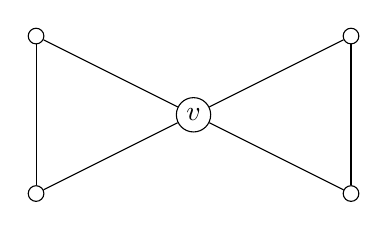
\begin{tikzpicture}
								\tikzstyle{vertex}=[circle,draw=black,minimum size=5pt,inner sep=2pt]
								\node[vertex] (1) at (0,0) {$v$};
								\node[vertex] (2) at (2,1) {};
								\node[vertex] (3) at (2,-1) {};
								\node[vertex] (4) at (-2,1) {};
								\node[vertex] (5) at (-2,-1) {};
								\draw (1) -- (3);
								\draw (1) -- (2);
								\draw (3) -- (2);
								\draw (1) -- (4);
								\draw (1) -- (5);
								\draw (4) -- (5);
							\end{tikzpicture}
						\end{center}
						此时$v$在一个环内,而若移去$v$,则$G$会成为非连通图,因此$v$是一个割点.
					\subsubsection*{(b)}
						不同意.反例如下:
						\begin{center}
							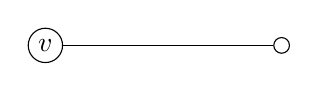
\begin{tikzpicture}
							\tikzstyle{vertex}=[circle,draw=black,minimum size=5pt,inner sep=2pt]
							\node[vertex] (1) at (0,0) {$v$};
							\node[vertex] (2) at (3,0) {};
							\draw (1) -- (2);
							\end{tikzpicture}
						\end{center}
						此时$v$不在任何环内,而$v$不是割点.
					\subsubsection*{(c)}
						不同意.反例如下:
						\begin{center}
							\begin{tikzpicture}
							\tikzstyle{vertex}=[circle,draw=black,minimum size=5pt,inner sep=2pt]
							\node[vertex] (1) at (0,0) {$v$};
							\node[vertex] (2) at (0,2) {};
							\node[vertex] (3) at (0,-2) {};
							\node[vertex] (4) at (-2,0) {};
							\node[vertex] (5) at (2,0) {};
							\draw (1) -- (2);
							\draw (1) -- (3);
							\draw (1) -- (4);
							\draw (1) -- (5);
							\end{tikzpicture}
						\end{center}
						此时割点有1个,端点有4个,割点少于端点.
					\subsubsection*{(d)}
						再次借用(c)中的图,其割点有1个,而桥边有4条,割点数少于桥边数.
				\subsection*{5.4}
					\begin{proof}
						因为$v$是图$G$的割点,所以$G-v$不连通,至少有两个连通分量.在$G-v$中任取两结点$v_1,v_2$,若两者处于不同连通分量,则在$\overline{G}$中两者连通;若两者处于同一连通分量,在其他分量中取一结点$v_3$,于是在$\overline{G}$中$v_1,v_2$相连.因此$v$不是$\overline{G}$的割点.
					\end{proof}
				\subsection*{5.6}
					\begin{proof}
						首先,若3-正则图$G$有一个割点$v$,先证其存在不在环中的边:若所有边都在环中,由于每个结点的度数都为3,当移去$v$后对任意两个结点仍然有相连的路径.因此存在不在环中的边,该边即为桥.\\
						再者,如果$G$有桥,显然$G$的结点个数大于等于3,由Corollary 5.2可知$G$包含一个割点.
					\end{proof}
				\subsection*{5.10}
					\begin{proof}
						如果边数不少于2的连通图$G$是不可分图,假设存在两条相邻的边$uv,vw$属于不同的两个环,且$u->w$的唯一路径经过$v$(若存在其他路径,则两边属于同一环).选取$v$,此时$G-v$将$u$和$w$分在不同的分量中,这与$G$是不可分图矛盾.因此任意两条相邻边都属于同一个环.\\
						如果$G$中任意两条相邻边都属于同一个环,则取任意一对相邻边$uv,vw$,$u,v,w$都不可能是割点.因此$G$是不可分图.
					\end{proof}
				\subsection*{5.11}
					\begin{proof}
						假设$G$可分,即存在一个割点$v$,且至少有两个块,$G-v$至少有两个连通分量.对于每个连通分量中的结点,取结最少的连通分量,则假若该分量中每个结点的度数都大于等于$\frac{n}{2}$,则该分量中至少有$\frac{n}{2}$个结点,加之$v$,则原先图$G$中至少有$n+1$个结点,不成立.因此$G$不可分.
					\end{proof}
				\subsection*{5.14}
					\subsubsection*{(a)}
						由于$G_1$是$G-v$的一个连通分量,所以$G_1$是连通图,显然$G[V(G_1)]$是连通图.假设$G_1$中不存在结点$u$,使得在$G$中$u$和$v$连通,则与$G$是连通图矛盾.故存在这样的结点$u$,于是诱导子图$G[V(G_1)\cup\{v\}]$是连通图.
					\subsubsection*{(b)}
						举例如下:
						\begin{center}
							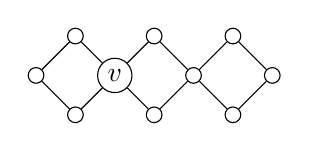
\begin{tikzpicture}
							\tikzstyle{vertex}=[circle,draw=black,minimum size=5pt,inner sep=2pt]
							\node[vertex] (1) at (-0.5,0.5) {};
							\node[vertex] (2) at (-0.5,-0.5) {};
							\node[vertex] (3) at (0,0) {$v$};
							\node[vertex] (4) at (0.5,0.5) {};
							\node[vertex] (5) at (0.5,-0.5) {};
							\node[vertex] (6) at (1,0) {};
							\node[vertex] (7) at (1.5,0.5) {};
							\node[vertex] (8) at (1.5,-0.5) {};
							\node[vertex] (9) at (2,0) {};
							\node[vertex] (10) at (-1,0) {};
							\draw (1) -- (10);
							\draw (2) -- (10);
							\draw (1) -- (3);
							\draw (2) -- (3);
							\draw (3) -- (4);
							\draw (3) -- (5);
							\draw (6) -- (4);
							\draw (6) -- (5);
							\draw (6) -- (7);
							\draw (6) -- (8);
							\draw (9) -- (8);
							\draw (9) -- (7);
							\end{tikzpicture}
						\end{center}
						选右边的一个连通分量,易知该诱导子图不是$G$的一个块,因此不必要.
				\subsection*{5.15}
					\begin{proof}
						先证(1)->(2):\\
						若$G_1$是$G$中的一个不可分的子图且不是其他任何$G$的不可分子图的真子集,假设$G_1$中存在不满足Theorem 5.8中等价关系的两条边,其不属于同一个环,由题5.10的证明知$G_1$可分,与条件矛盾.故推得(2).\\
						再证(2)->(1):\\
						若G由那些满足Theorem 5.8中等价关系的边对诱导而成,则对于任意一条边总能找到与其同在一个环中的另一条边,满足不可分的性质.假设存在一个$G$的不可分子集$G_2$,使得$G_1\subset G_2$,则$G_2$比$G_1$多的边无法与其他边成环(否则违背条件),故存在桥,于是便可分,与不可分矛盾.故推得(1).
					\end{proof}
				\subsection*{5.20}
					\subsubsection*{(a)}
						\begin{proof}
							因为$n=4,2\le k\le n-2$,故$k=2$.若$G$不是2-connected图,则存在一个结点$v$,$G-v$是非连通图,便可知$G$包含一个vertex-cut$U$且$|U|=k-1$.
						\end{proof}
					\subsubsection*{(b)}
						\begin{proof}
							若$G$不是2-edge-connected图,则存在一条边$uv$,$G-{uv}$是连通图,便可知$G$包含一个edge-cut$X$且$|X|=k-1$.
						\end{proof}
				\subsection*{5.22}
					\subsubsection*{(a)}
						\begin{proof}
							若$G$是一个k-connected图,则去掉任意$k-1$个结点,仍然保持连通性.假设去掉的边$e$连接去掉的两个结点,则对结果无影响,仍可满足k-connected.若$e$连接去掉的结点和没有去掉的结点,同理可满足k-connected.若$e$连接没有去掉的两个结点,只要保留其中一个结点即可,于是条件可放宽至(k-1)-connected.因此$G-e$是(k-1)-connected.
						\end{proof}
					\subsubsection*{(b)}
						\begin{proof}
							若$G$是一个k-edge-connected图,则去掉任意$k-1$条边,仍然保持连通性.若$e$是先前去掉的边之一,则不影响结果,仍满足k-edge-connected.若是新去掉的边,则保留该边即可,因此$G-e$是(k-1)-edge-connected.
						\end{proof}
				\subsection*{5.30}
					$\overline{\kappa}(G)\ge\kappa(G),\overline{\lambda}(G)\ge\lambda(G),\overline{\kappa}(G)\le\overline{\lambda}(G)$.
			\section*{GC Chapter 6}
				\subsection*{6.4}
					\subsubsection*{(a)}
					\begin{center}
						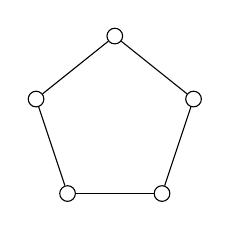
\begin{tikzpicture}
						\tikzstyle{vertex}=[circle,draw=black,minimum size=5pt,inner sep=2pt]
						\node[vertex] (1) at (0,0) {};
						\node[vertex] (2) at (-1,-0.8) {};
						\node[vertex] (3) at (1,-0.8) {};
						\node[vertex] (4) at (-0.6,-2) {};
						\node[vertex] (5) at (0.6,-2) {};
						\draw (1) -- (2);
						\draw (1) -- (3);
						\draw (2) -- (4);
						\draw (3) -- (5);
						\draw (4) -- (5);
						\end{tikzpicture}
					\end{center}
					补图:五角星.
					\subsubsection*{(b)}
					\begin{center}
						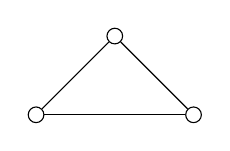
\begin{tikzpicture}
						\tikzstyle{vertex}=[circle,draw=black,minimum size=5pt,inner sep=2pt]
						\node[vertex] (1) at (0,0) {};
						\node[vertex] (2) at (-1,-1) {};
						\node[vertex] (3) at (1,-1) {};
						\draw (1) -- (2);
						\draw (1) -- (3);
						\draw (2) -- (3);
						\end{tikzpicture}
					\end{center}
					\subsubsection*{(c)}
					\begin{center}
						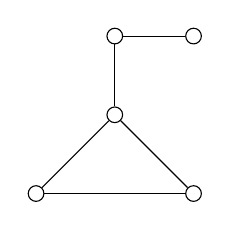
\begin{tikzpicture}
						\tikzstyle{vertex}=[circle,draw=black,minimum size=5pt,inner sep=2pt]
						\node[vertex] (1) at (0,0) {};
						\node[vertex] (2) at (0,1) {};
						\node[vertex] (3) at (1,1) {};
						\node[vertex] (4) at (-1,-1) {};
						\node[vertex] (5) at (1,-1) {};
						\draw (1) -- (2);
						\draw (2) -- (3);
						\draw (1) -- (4);
						\draw (1) -- (5);
						\draw (4) -- (5);
						\end{tikzpicture}
					\end{center}
					补图:
					\begin{center}
						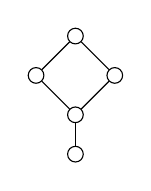
\begin{tikzpicture}
						\tikzstyle{vertex}=[circle,draw=black,minimum size=5pt,inner sep=2pt]
						\node[vertex] (1) at (0,0) {};
						\node[vertex] (2) at (-0.5,-0.5) {};
						\node[vertex] (3) at (0.5,-0.5) {};
						\node[vertex] (4) at (0,-1) {};
						\node[vertex] (5) at (0,-1.5) {};
						\draw (1) -- (2);
						\draw (1) -- (3);
						\draw (2) -- (4);
						\draw (3) -- (4);
						\draw (4) -- (5);
						\end{tikzpicture}
					\end{center}
					\subsubsection*{(d)}
					\begin{center}
						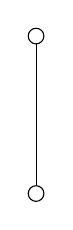
\begin{tikzpicture}
						\tikzstyle{vertex}=[circle,draw=black,minimum size=5pt,inner sep=2pt]
						\node[vertex] (1) at (0,0) {};
						\node[vertex] (2) at (0,2) {};
						\draw (1) -- (2);
						\end{tikzpicture}
					\end{center}
					\subsubsection*{(e)}
					\begin{center}
					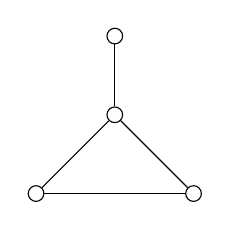
\begin{tikzpicture}
					\tikzstyle{vertex}=[circle,draw=black,minimum size=5pt,inner sep=2pt]
					\node[vertex] (1) at (0,0) {};
					\node[vertex] (2) at (0,1) {};
					\node[vertex] (3) at (-1,-1) {};
					\node[vertex] (4) at (1,-1) {};
					\draw (1) -- (2);
					\draw (1) -- (3);
					\draw (1) -- (4);
					\draw (3) -- (4);
					\end{tikzpicture}
					\\去掉最上方的边即可构成欧拉图.
				\end{center}
				\subsection*{6.5}
				\begin{center}
					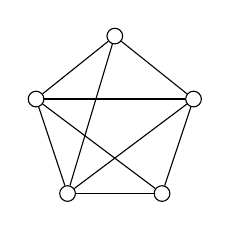
\begin{tikzpicture}
					\tikzstyle{vertex}=[circle,draw=black,minimum size=5pt,inner sep=2pt]
					\node[vertex] (1) at (0,0) {};
					\node[vertex] (2) at (-1,-0.8) {};
					\node[vertex] (3) at (1,-0.8) {};
					\node[vertex] (4) at (-0.6,-2) {};
					\node[vertex] (5) at (0.6,-2) {};
					\draw (1) -- (2);
					\draw (1) -- (3);
					\draw (1) -- (4);
					\draw (2) -- (3);
					\draw (2) -- (4);
					\draw (2) -- (5);
					\draw (3) -- (5);
					\draw (3) -- (4);
					\draw (4) -- (5);
					\end{tikzpicture}
				\end{center}
				\subsection*{6.6}
				\begin{proof}
					由于$G$是正则图,则每个结点的度数都相同,设为$k$.由于$G$连通且不是欧拉图,则$k$为奇数.$k$正则图存在的必要和充分条件是$n\ge k+1$并且$nk$是偶数,因此$n$为偶数.在$\overline{G}$中,每个结点的度数变为$n-1-d$为偶数.又因为其连通,所以是欧拉图.
				\end{proof}
				\subsection*{6.13}
					\subsubsection*{(a)}
						\begin{center}
							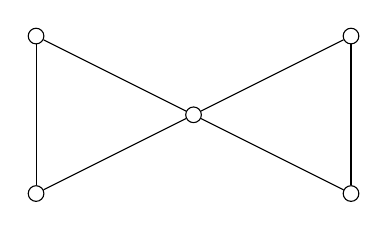
\begin{tikzpicture}
							\tikzstyle{vertex}=[circle,draw=black,minimum size=5pt,inner sep=2pt]
							\node[vertex] (1) at (0,0) {};
							\node[vertex] (2) at (2,1) {};
							\node[vertex] (3) at (2,-1) {};
							\node[vertex] (4) at (-2,1) {};
							\node[vertex] (5) at (-2,-1) {};
							\draw (1) -- (3);
							\draw (1) -- (2);
							\draw (3) -- (2);
							\draw (1) -- (4);
							\draw (1) -- (5);
							\draw (4) -- (5);
							\end{tikzpicture}
						\end{center}
						不存在能够经过所有顶点的环.
					\subsubsection*{(b)}
						\begin{center}
							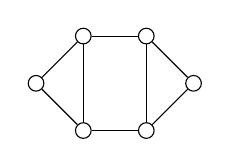
\begin{tikzpicture}
							\tikzstyle{vertex}=[circle,draw=black,minimum size=5pt,inner sep=2pt]
							\node[vertex] (1) at (0,0) {};
							\node[vertex] (2) at (-0.6,-0.6) {};
							\node[vertex] (3) at (0,-1.2) {};
							\node[vertex] (4) at (0.8,0) {};
							\node[vertex] (5) at (1.4,-0.6) {};
							\node[vertex] (6) at (0.8,-1.2) {};
							\draw (1) -- (2);
							\draw (1) -- (3);
							\draw (3) -- (2);
							\draw (1) -- (4);
							\draw (5) -- (6);
							\draw (4) -- (5);
							\draw (4) -- (6);
							\draw (3) -- (6);
							\end{tikzpicture}
						\end{center}
						存在度数为奇数的结点,故不是欧拉图.
					\subsubsection*{(c)}
						\begin{center}
							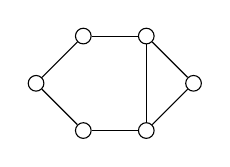
\begin{tikzpicture}
							\tikzstyle{vertex}=[circle,draw=black,minimum size=5pt,inner sep=2pt]
							\node[vertex] (1) at (0,0) {};
							\node[vertex] (2) at (-0.6,-0.6) {};
							\node[vertex] (3) at (0,-1.2) {};
							\node[vertex] (4) at (0.8,0) {};
							\node[vertex] (5) at (1.4,-0.6) {};
							\node[vertex] (6) at (0.8,-1.2) {};
							\draw (1) -- (2);
							\draw (3) -- (2);
							\draw (1) -- (4);
							\draw (5) -- (6);
							\draw (4) -- (5);
							\draw (4) -- (6);
							\draw (3) -- (6);
							\end{tikzpicture}
						\end{center}
					\subsubsection*{(d)}
					\begin{center}
						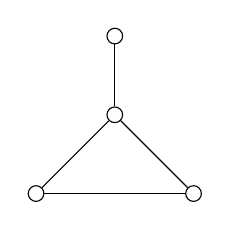
\begin{tikzpicture}
						\tikzstyle{vertex}=[circle,draw=black,minimum size=5pt,inner sep=2pt]
						\node[vertex] (1) at (0,0) {};
						\node[vertex] (2) at (0,1) {};
						\node[vertex] (3) at (-1,-1) {};
						\node[vertex] (4) at (1,-1) {};
						\draw (1) -- (2);
						\draw (1) -- (3);
						\draw (1) -- (4);
						\draw (3) -- (4);
						\end{tikzpicture}
					\end{center}
				\subsection*{6.16}
					\subsubsection*{(a)}
						\begin{proof}
							若$\overline{G}$不是欧拉图,则$n-1-r$为奇数,又因为$n$为偶数,故$r$是偶数,又$G$连通,因此$G$是欧拉图;\\
							若$G$不是欧拉图,则$r$为奇数,如此$n-1-r$为偶数,推得$\overline{G}$是欧拉图.得证.
						\end{proof}
					\subsubsection*{(b)}
						\begin{proof}
							若$G$不是汉密尔顿图,则存在$G$中的结点$v$,其$deg(v)<\frac{n}{2}$,又因为其为正则图,故所有的结点的度数都小于$\frac{n}{2}$,其补图$\overline{G}$的每个结点的度数都大于等于$\frac{n}{2}$,由此可推知$\overline{G}$是汉密尔顿图.\\
							若$\overline{G}$不是汉密尔顿图,则仿照上方证明易推知$G$是汉密尔顿图.得证.
						\end{proof}
				\subsection*{6.21}
					假设对任意不相邻的结点$u,v$,都有$degu+degv\ge n$,则$G$为汉密尔顿图,显然有汉密尔顿路径\\
					假设存在两个不相邻的结点$u,v$,且$degu+degv=n-1$,则通过添加一条边$uv$,即可满足$degu+degv=n$,而此时亦可满足汉密尔顿图.而汉密尔顿图通过去掉某条边亦可以满足汉密尔顿路径.如此,对于每一对非相邻且度数和为$n-1$的结点如此操作,即可证得$G$包含一条汉密尔顿路径.
			
		\end{SChinese}
	\end{CJK}
\end{document}